
\begin{frame}[plain]
  \titlepage
\end{frame}




\section{Введение}

\begin{frame}
    {Структура рецептора}
	\begin{center}
          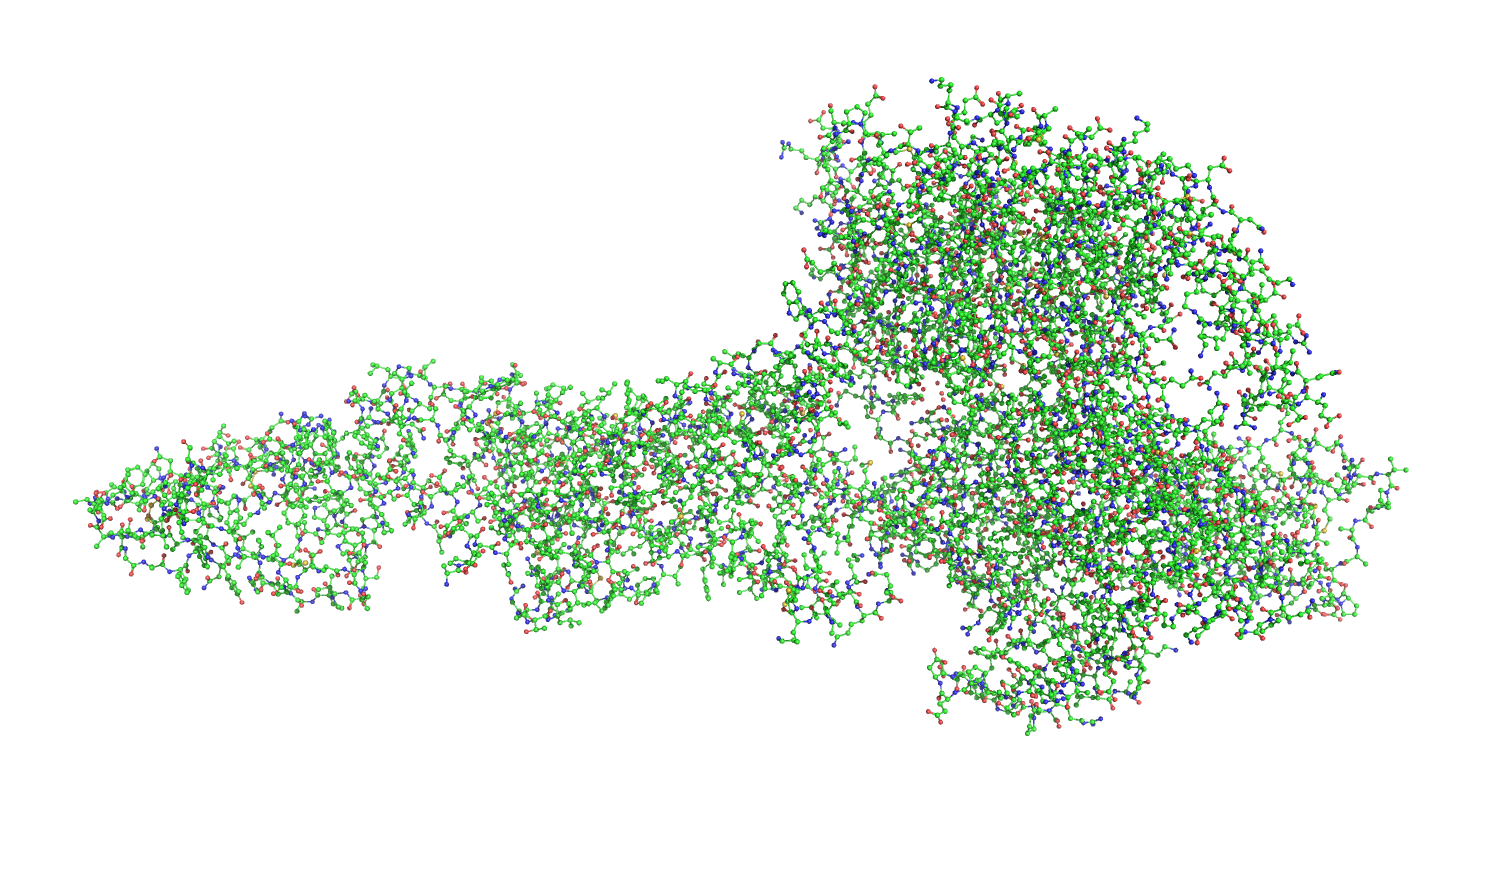
\includegraphics[width=0.85\textwidth]{prot.png}
	  \end{center}
  \end{frame}


\begin{frame}
    {Что такое белок?}{}
	\textbf{Белки}  — высокомолекулярные органические вещества, состоящие из соединённых в цепочку пептидной связью альфа-аминокислот.(wikipedia) \\
	\vspace{.5cm}
	\begin{center}
	\small%
	\chemfig[atom sep=2em]{-N(-[2]H)-C(-[2]H)(-[6]R_1)-C(=[2]O)-N(-[6]H)-C(-[6]H)(-[2]R_2)-C(=[6]O)-N(-[2]H)-C(-[2]H)(-[6]R_3)-C(=[2]O)-}\\
	\vspace{.5cm}
    \end{center}
	\textbf{Или:} белок это линейный полярный полимер, где мономерами является выборка из примерно 20 L-альфа-аминокислот. 

\end{frame}

\setchemfig{atom sep=2em, cram width=0.2em}

\begin{frame}
    {Что такое  L альфа-аминокислота?}{}
	\begin{center}
%\setatomsep{2.7em}\setcrambond{0.2em}{}{}%
 \chemfig{C(-[5]H)(-[2]H)(<[:-60]H)(<:[:-20]H)} \\
 \small
 атом углерода в $sp^3$ гибридизации имеет тетраэдрическое окружение\\
  \vspace{.5cm}
 \chemfig{C(-[5]NH)(-[7]CO)(<[:60]R_1)(<:[:120]H)}
 \hspace{1cm}
 \chemfig{C(-[5]NH)(-[7]CO)(<:[:60]R_1)(<[:120]H)}\\
 \vspace{.2cm}
 L-аминокислота \hspace{1cm} D-аминокислота \\
 \end{center}
% \chemfig{C(-[5]NH)(-[2]R_1)(<[:-60]CO)(<:[:-20]H)}
\end{frame}

\begin{frame}
    {Аминокислоты}
	\begin{center}
          \includegraphics[width=.9\textwidth]{Amino_Acids}
          %[height=.7\textheight]{Amino_Acids}
    \end{center}
  \end{frame}


\begin{frame}
    {Пептидная связь}
	\begin{center}
%		         \setlength{\fboxsep}{1pt}
%				            \fcolorbox{black}{white}{ 
%          \includegraphics[width=.8\textwidth]{pep1.eps}
  \begin{tikzpicture}[help lines/.style={thin,draw=black!50}]
%  \draw[help lines] (0,0) grid (8,4);    
   \node (2) at (4,2) {
   % \schemedebug{true}
     %\setatomsep{2.7em}\setcrambond{0.2em}{}{}%
     %\setbondstyle{line width=1pt}
     \chemfig{
         H_2N-[1](-[2]R_1)-[7]C(=[6]O)-[1,,,,white!40!blue,{line width=2pt}]N(-[2]H)-[7](-[6]R_2)-[1]C(=[2]O)-[7,,,,white!40!blue,{line width=2pt}]N(-[6]H)
         -[1](-[2]R_3)-[7]C(=[6]O)-[1]OH
         }
	  };
      \draw[orange] (1.5,1.8) ellipse (1.3cm and 2cm);
      \draw[orange] (3.7,2.3) ellipse (1.2cm and 2cm);
      \draw[orange] (5.9,1.8) ellipse (1.2cm and 2cm);
      \node (pep) at (4,-1) {Пептидные связи};
      \draw [->,white!40!blue,thick] (pep.north) -- (2.8,2);
      \draw [->,white!40!blue,thick] (pep.north) -- (4.8,2);
      %node[ellipse, minimum height=4cm,minimum width=2cm,draw] {};
  \end{tikzpicture}
 \end{center}
\end{frame}

\begin{frame}
    {Пептидная связь, таутомерия}
	\begin{center}
	 \schemestart
	 \small%
%		 \setatomsep{2em}%
%\setatomsep{2.7em}\setcrambond{0.2em}{}{}%
	 \chemfig{C(-[5])(<:[:60]H)(<[:120]R_1)-[7]C(=[6]O)-[1,,,,white!40!blue,{line width=1pt}]N(-[2]H)-[7]C(<:[:-60]R_2)(<[:-120]H)-[1] }%
	 \arrow{<=>}%
%\setatomsep{2.7em}\setcrambond{0.2em}{}{}%
	 \small\chemfig{C(-[5])(<:[:60]H)(<[:120]R_1)-[7]C(-[6]OH)=[1,,,,white!40!red,{line width=1pt}]N-[7]C(<:[:-60]R_2)(<[:-120]H)-[1] }%
	  \schemestop
    \end{center}
\end{frame}

\begin{frame}
{Пептидная связь, свойства}
	\begin{itemize}
		\item Пептидная связь прочнее, чем другие амиды
		\item Атомы пептидного звена ( C$_\alpha$-C-N- C$_\alpha$) лежат в одной плоскости
    \item Валентные углы у атомов С и N примерно равны $120^o$
		\item Вращение вокруг связи C-N затруднено
		\item Возможны cis- и trans-конфигурации; в белках преобладают trans
		\item Карбонильный кислород – хороший акцептор водорода
		\item Амидный азот – хороший донор водорода
		\end{itemize}
 \end{frame}

 \begin{frame}
{Вращения вокруг связей в остове белка}
	\begin{center}
%`\setatomsep{3.7em}\setcrambond{0.2em}{}{}%
	 \chemfig{C(-[5])(<:[:60]H)(<[:120]R_1)-[7]C(=[6]O)-[@{om}1]N
     (-[2]H)-[@{phi}7]C(<:[:-60]R_2)(<[:-120]H)-[@{psi}1]C(=[2]O)-[7]}%
 \chemmove{%
     \draw[-stealth,thick,white!40!red]
     (phi).. controls +(45:5mm) and +(-90:5mm).. node[above right]
     {$\boldsymbol{\phi}$}(phi);
     \draw[-stealth,thick,white!40!blue]
     (psi).. controls +(135:5mm) and +(-90:5mm).. node[below right]
     {$\boldsymbol{\psi}$}(psi);
     \draw[-stealth,thick,green!60!black]
     (om).. controls +(135:5mm) and +(-90:5mm).. node[above left]
     {$\boldsymbol{\omega}$}(om);
 }
	  \end{center}
  \end{frame}




  \begin{frame}
{Вращения вокруг связей в остове белка}
	\begin{center}
%\setatomsep{3.7em}\setcrambond{0.2em}{}{}%
	 \chemfig{C(-[5])(<:[:60]H)(<[:120]R_1)-[7]C(=[6]O)-[@{om}1]N
     (-[2]H)-[@{phi}7]C(<:[:-60]R_2)(<[:-120]H)-[@{psi}1]C(=[2]O)-[7]}%
 \chemmove{%
     \draw[-stealth,thick,white!40!red]
     (phi).. controls +(45:5mm) and +(-90:5mm).. node[above right]
     {$\boldsymbol{\phi}$}(phi);
     \draw[-stealth,thick,white!40!blue]
     (psi).. controls +(135:5mm) and +(-90:5mm).. node[below right]
     {$\boldsymbol{\psi}$}(psi);
     \draw[-stealth,thick,green!60!black]
     (om).. controls +(135:5mm) and +(-90:5mm).. node[above left]
     {$\boldsymbol{\omega}$}(om);
 }
	  \end{center}

 $ \begin{array}{l}  \phi\\ \psi  \end{array}  \Bigg \} $ теоретически могут быть: от –180$^0$ до +180$^0$ \\
 \vspace{.5cm}
	  а $\omega$ ?
  \end{frame}

  \begin{frame}
{Карта Рамачандрана}
	  даже в полиглициновой цепи существуют стерические ограничения
	\begin{center}
          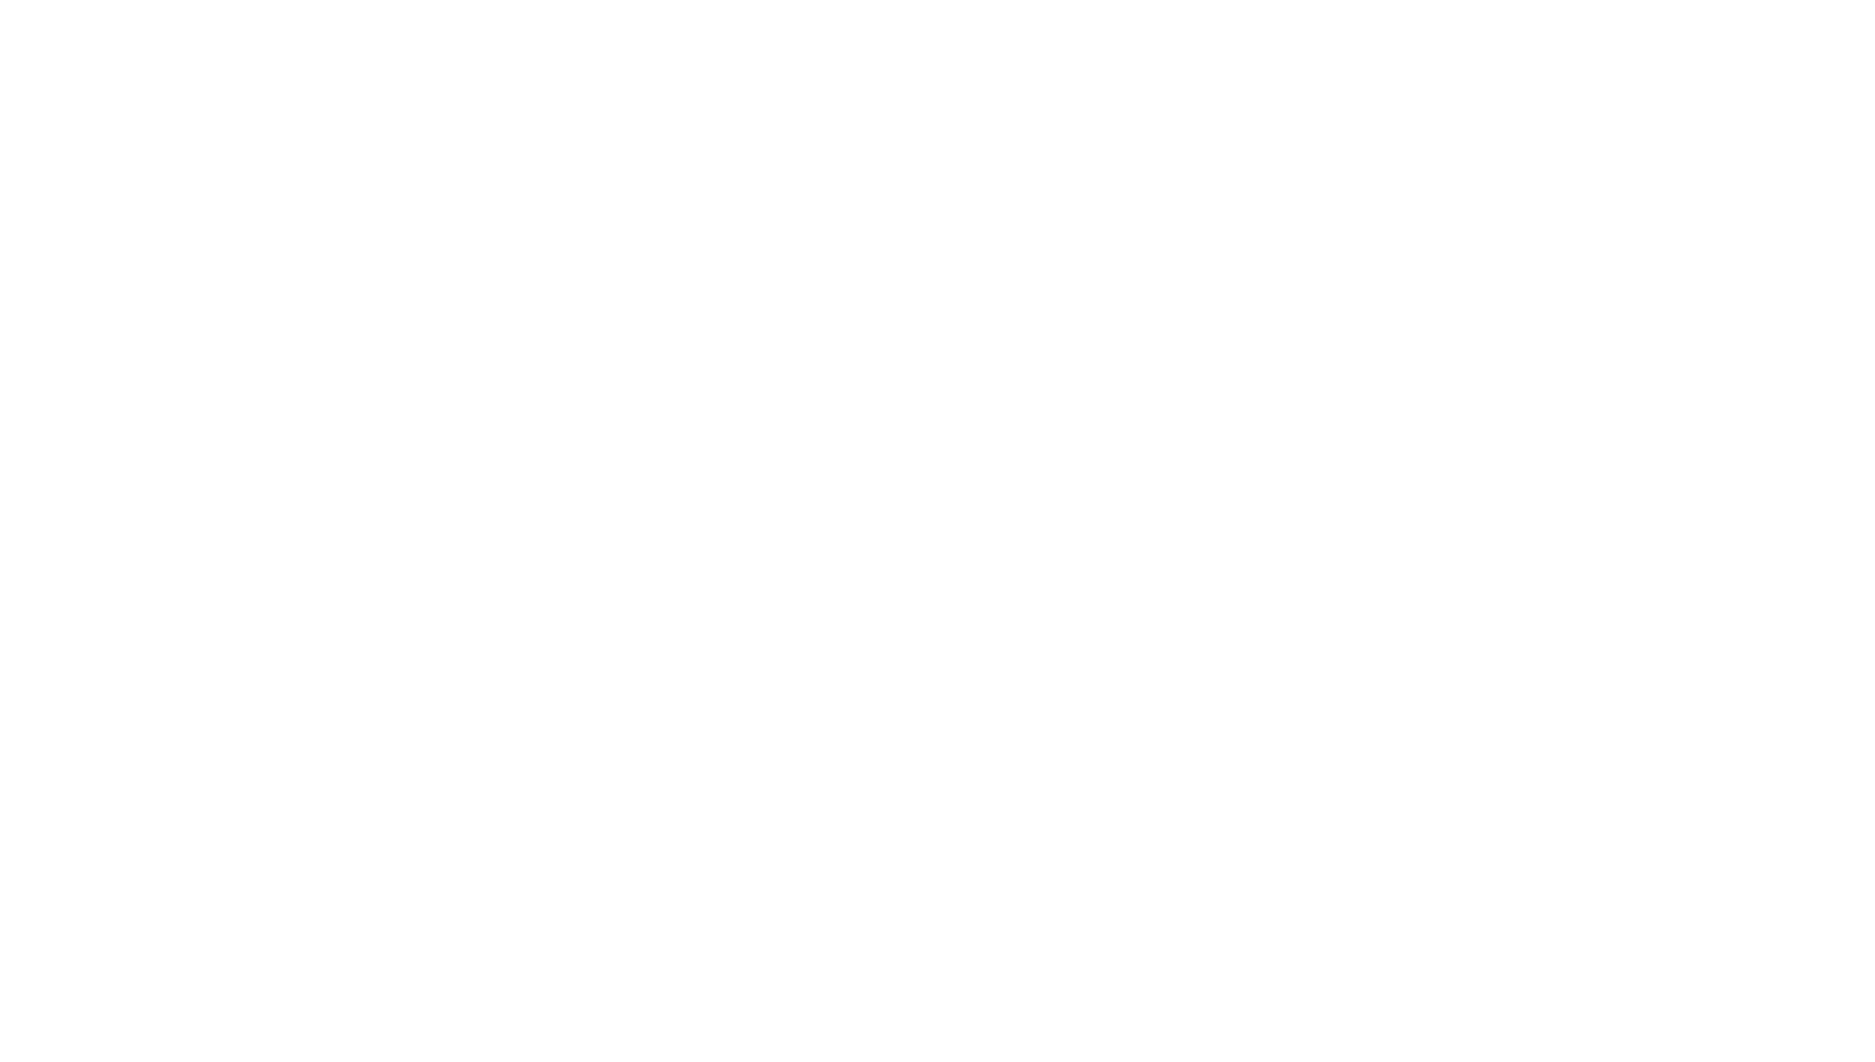
\includegraphics[width=0.75\textwidth]{ram_gly.png}
	  \end{center}
  \end{frame}
 
  \section{Уровни организации структуры белка}
  \begin{frame}
{Уровни организации структуры белка}
	  \begin{itemize}
		  \item Первичная структура
		  \item Вторичная структура
		  \item Укладка (fold)
		  \item Третичная структура
		  \item Четвертичная структура
		  \end{itemize}
	  \end{frame}

  \begin{frame}
{Первичная структура}
	  Первичная структура – это аминокислотная последовательность:\\
	  \vspace{.5cm}
	  Met-Ala-Gly-Trp-Ala-Val-Asp \ldots
  \end{frame}

  \begin{frame}
{Вторичная структура}
	  \begin{wrapfigure}{r}{2cm}
	  \includegraphics[width=2cm]{ab.png}\\
	  \includegraphics[width=2cm]{bturn.png}
      \end{wrapfigure}
	  \textbf{Вторичная структура белка} - это упорядоченные расположения атомов основной цепи полипептида, 	 безотносительно к типам боковых цепей (групп) и их конформациям.\\
	  \vspace{.5cm}
	  Если упорядоченность такова, что двугранные углы
	  одинаковы у всех остатков, то говорят о
	  регулярной вторичной структуре. Регулярными
	  вторичными структурами являются спирали и $\beta$–
	  структуры.\\
	  \vspace{.7cm}
	  Пример нерегулярной вторичной структуры 
	  $\beta$–поворот ($\beta$–изгиб, реверсивный поворот).
  \end{frame}


  \begin{frame}
{Регулярные вторичные структуры}
	\begin{center}
%		         \setlength{\fboxsep}{3pt}
%				            \fcolorbox{black}{white}{ 
          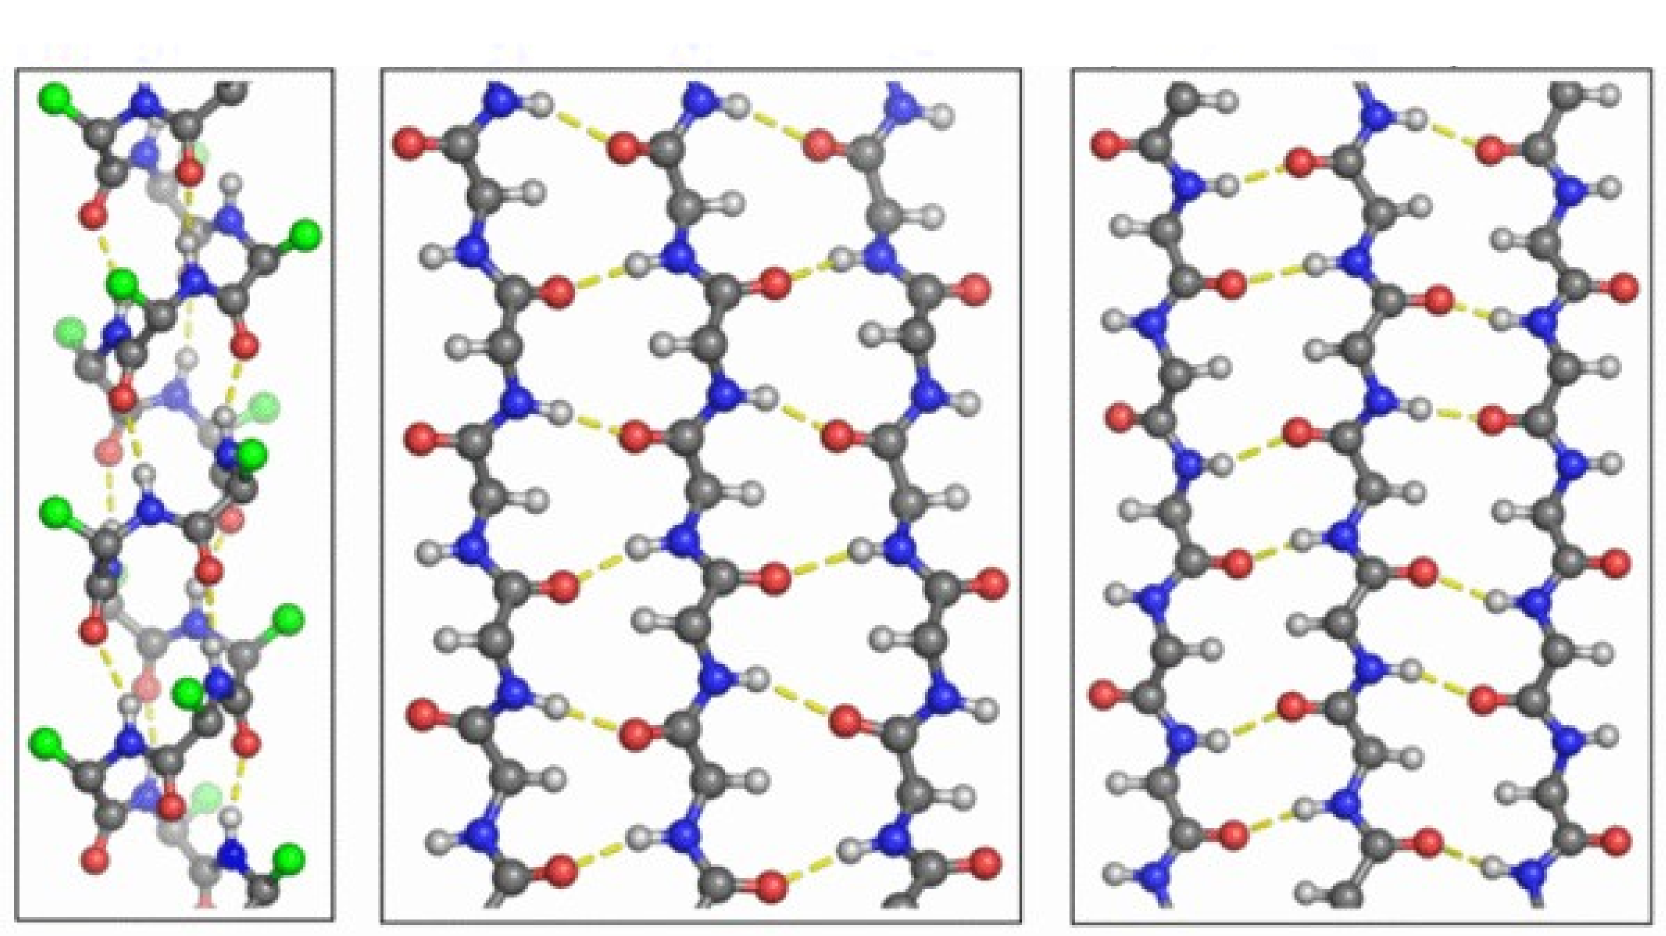
\includegraphics[width=0.8\textwidth]{ss.png}
%	  }
	  \end{center}
	\end{frame}

	\begin{frame}
{Укладка (fold)}
		Укладкой называют организацию в пространстве элементов регулярной вторичной структуры. \\
		Пример: $\alpha$ -спиральные белки\\
	\begin{center}
          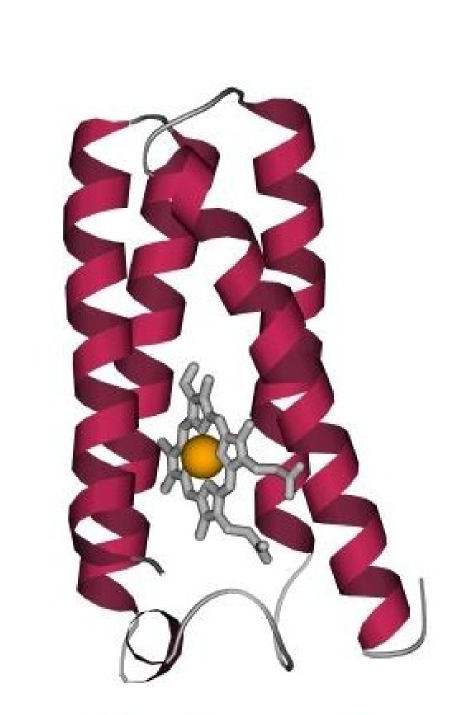
\includegraphics[width=0.2\textwidth]{ss1.png}
          
\includegraphics[width=0.2\textwidth]{ss2.png}
          \includegraphics[width=0.2\textwidth]{ss3.png}
	  \end{center}
	\end{frame}

\begin{frame}
{\texorpdfstring{$\beta$} - структурные белки}
	\begin{center}
		         %\setlength{\fboxsep}{0pt}
				  %          \fcolorbox{black}{white}{ 
								\begin{minipage}{\textwidth}
         % \includegraphics[width=0.5\textwidth]{b1.png}
         % \includegraphics[width=0.5\textwidth]{b2.png} \\
          \includegraphics[height=0.6\textheight]{b3.png}
          \includegraphics[height=0.6\textheight]{b4.png}
	  \end{minipage}
	  %}
	  \end{center}
	\end{frame}

	\begin{frame}
{Распределение в природе}
	\begin{center}
          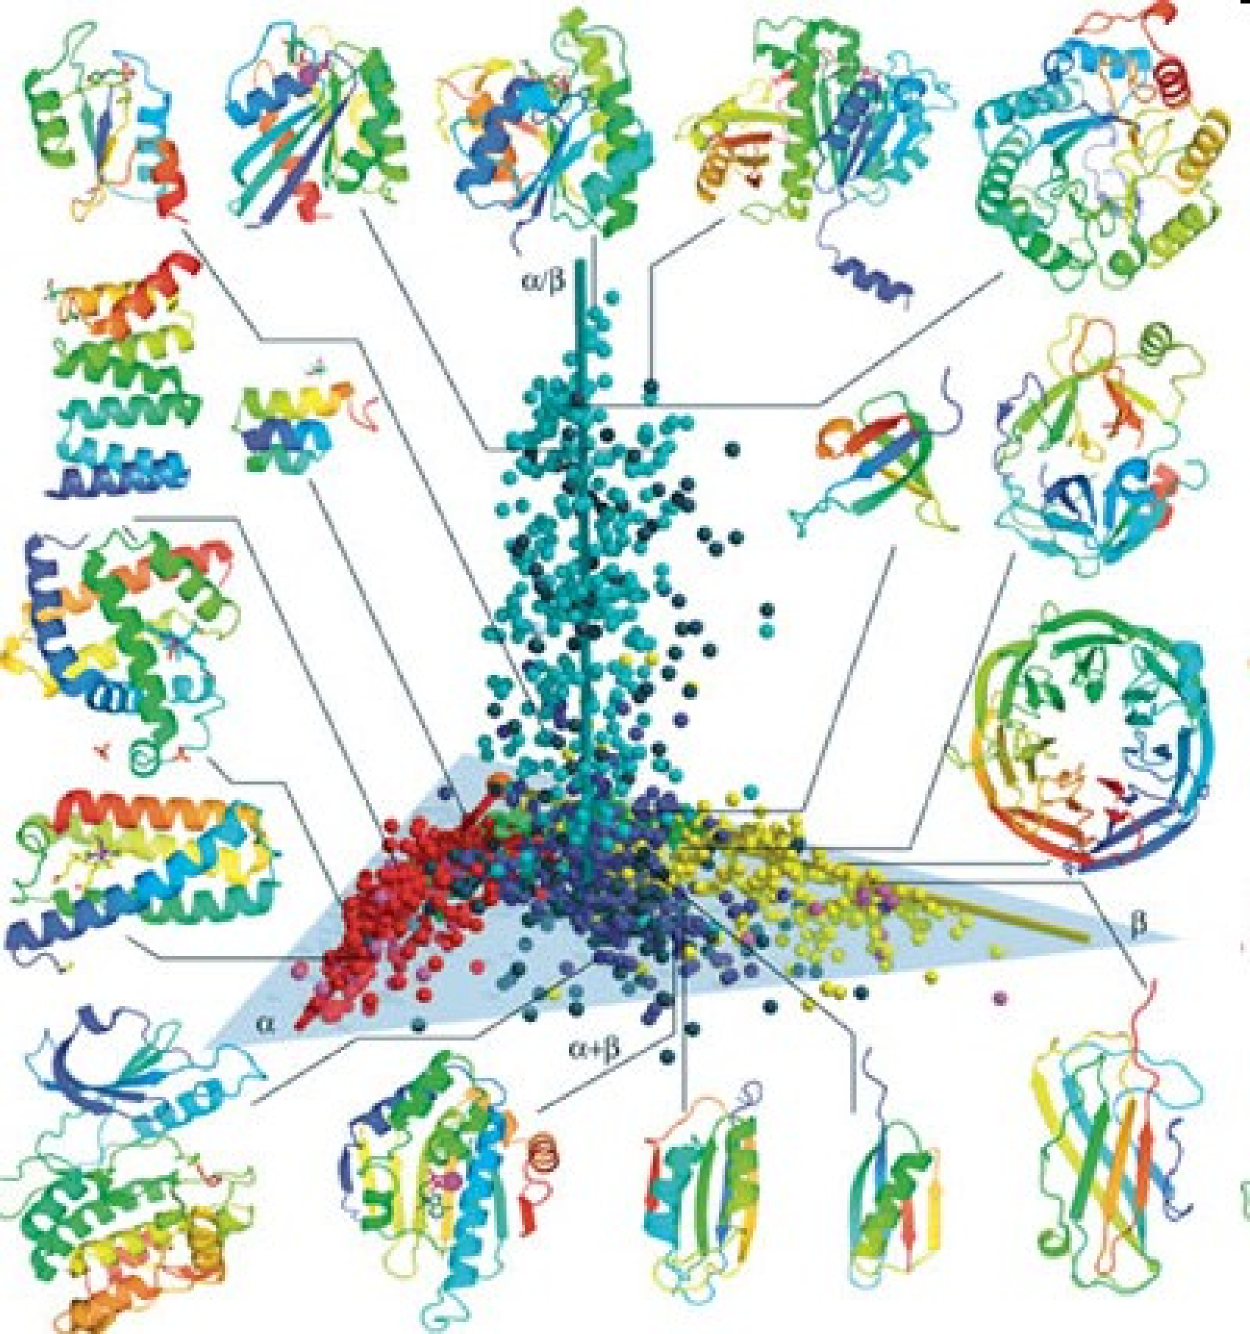
\includegraphics[width=0.4\textwidth]{scheme1.png}
	  \end{center}
	\end{frame}

	\begin{frame}
{Третичная структура}
		Третичной структурой называют расположение в пространстве всех атомов
		одной полипептидной цепи. \\
		Т.e. описание третичной структуры включает в себя:
		\begin{itemize}
			\item описание элементов вторичной структуры,
			\item описание типа укладки,
			\item описание структуры петель,
			\item описание конформаций боковых групп всех аминокислотных остатков.
			\end{itemize}
		\end{frame}
\section{Типы взаимодействий в белках}

\begin{frame}
{Вспомогательные взаимодействия: водородные связи}
	\begin{center}
        \chemfig{
            -[5]N-[7]C_\alpha(-[5]C(-[7])=[4]O)--[1]@{o1}O-H
            -[7,,,,dashed]@{o2}\Charge{120=\:,-120=\:}{O}=C(-[::60]\Charge{60=\-}{O})-[::-60]--[::-60]
        }
  \chemmove[dashed,white!40!red]{
  \draw[->] (o1) -- (o2)  node[below left] {3.5\AA\hspace{1cm}~};}

		%         \setlength{\fboxsep}{3pt}
	%			            \fcolorbox{black}{white}{ 
    %      \includegraphics[width=0.7\textwidth]{hbond.eps}
	%  }
	  \end{center}
  \end{frame}

\begin{frame}
{Ионные пары}
	\begin{center}
        \chemfig{
            --[1]--[7]@{o1}\chemabove{NH_3}{\oplus}
            -[:-90,1.5,,,draw=none,white!40!red]@{o3}\Charge{120=\:,-120=\:}{O}=[::90]C(-[::60]@{o2}O^{-})
            -[::-60]-[::60]-[::-60]
        }
  \chemmove[dashed,white!40!red]{
  \draw[->] (o1) -- (o2)  node[below left] {~};
  \draw[->] (o1) -- (o3)  node[below left] {3.1\AA\hspace{1cm}~};}
	  \end{center}
  \end{frame}

\begin{frame}
{Дисульфидные мостики характерны для секретируемых белков}
	\begin{center}
        \chemfig{
            -[5]N-[7]C_\alpha(-[5]C(-[7])=[4]O)--[1]S-[0,,,,yellow!60!black,
            thick]S-[7]
            -[0]C_\alpha(-[1])-[7]
        }
	  \end{center}
  \end{frame}

\begin{frame}
{Гидрофобные взаимодействия – главный 	фактор, заставляющий глобулу свертываться}
	\begin{center}
  \begin{tikzpicture}[help lines/.style={thin,draw=black!50}]
  %\draw[help lines] (0,0) grid (8,4);    
   \node (2) at (4,2) {
     \chemfig{
         (-[1,0.5,,,draw=none]-[1,2,,,decorate,decoration=snake]COO^{-})
         (-[2,0.5,,,draw=none]-[2,2,,,decorate,decoration=snake]COO^{-})
         (-[0,0.5,,,draw=none]-[0,2,,,decorate,decoration=snake]COO^{-})
         (-[7,0.5,,,draw=none]-[7,2,,,decorate,decoration=snake]COO^{-})
         (-[5,0.5,,,draw=none]-[5,2,,,decorate,decoration=snake]^{-}OOC)
         (-[3,0.5,,,draw=none]-[3,2,,,decorate,decoration=snake]^{-}OOC)
         (-[4,0.5,,,draw=none]-[4,2,,,decorate,decoration=snake]^{-}OOC)
         (-[6,0.5,,,draw=none]-[6,2,,,decorate,decoration=snake]COO^{-})
 }};
      \draw[orange] (4,2) ellipse (2cm and 2cm);
      \node (pep) at (5,0) {$\approx$ 4\AA};
 \end{tikzpicture}

	  \end{center}
  \end{frame}




\begin{frame}
{От четвертичной структуры к молекулярным машинам}
	\begin{center}
%		         \setlength{\fboxsep}{0pt}
%				            \fcolorbox{black}{white}{ 
          \includegraphics[height=0.6\textheight]{4s1.png}
          \includegraphics[height=0.6\textheight]{4s2.png}
%	  }
	  \end{center}
  \end{frame}
	


